\iffalse
\let\negmedspace\undefined
\let\negthickspace\undefined
\documentclass[journal,12pt,twocolumn]{IEEEtran}
\usepackage{cite}
\usepackage{amsmath,amssymb,amsfonts,amsthm}
\usepackage{algorithmic}
\usepackage{graphicx}
\usepackage{textcomp}
\usepackage{xcolor}
\usepackage{txfonts}
\usepackage{listings}
\usepackage{enumitem}
\usepackage{mathtools}
\usepackage{gensymb}
\usepackage{comment}
\usepackage[breaklinks=true]{hyperref}
\usepackage{tkz-euclide} 
\usepackage{listings}
\usepackage{gvv}                                        
\def\inputGnumericTable{}                                 
\usepackage[latin1]{inputenc}                               \usepackage{caption}
\usepackage{color}                                            
\usepackage{array}                                            
\usepackage{longtable}                                       
\usepackage{calc}                                             
\usepackage{multirow}                                         
\usepackage{hhline}                                           
\usepackage{ifthen}                                           
\usepackage{lscape}

\newtheorem{theorem}{Theorem}[section]
\newtheorem{problem}{Problem}
\newtheorem{proposition}{Proposition}[section]
\newtheorem{lemma}{Lemma}[section]
\newtheorem{corollary}[theorem]{Corollary}
\newtheorem{example}{Example}[section]
\newtheorem{definition}[problem]{Definition}
\newcommand{\BEQA}{\begin{eqnarray}}
\newcommand{\EEQA}{\end{eqnarray}}
\newcommand{\define}{\stackrel{\triangle}{=}}
\theoremstyle{remark}
\newtheorem{rem}{Remark}
\begin{document}

\bibliographystyle{IEEEtran}
\vspace{3cm}

\title{NCERT 11.15. Q10}
\author{EE23BTECH11010 - Venkatesh Bandawar$^{*}$% <-this % stops a space
}
\maketitle
\newpage
\bigskip

\renewcommand{\thefigure}{\arabic{figure}}
\renewcommand{\thetable}{\arabic{table}}

\bibliographystyle{IEEEtran}

\parindent 0px
\textbf{Question:} For the travelling harmonic wave
$y\brak {x, t} = 2.0 \cos 2\pi \brak{10t - 0.0080 x + 0.35}$ where $x$ and $y$ are in $cm$ and $t$ in $s$. Calculate the phase difference between oscillatory
motion of two points separated by a distance of 

\begin{enumerate} [label=(\alph*)]
    \item $4 m$
    \item $0.5 m$
    \item $\lambda/2$
    \item $3\lambda/4$
\end{enumerate}

\solution
\fi
\begin{table}[htbp] \small
\centering
\begin{tabular}{|c|c|c|}
\hline
\textbf{Parameter}&\textbf{Description} &\textbf{Value}\\
   \hline
    $y\brak{x_i, t}$ & \parbox{3cm}{equation of harmonic wave\vphantom{\brak{0.1}}} & $A \cos \brak{2\pi f t - k x_i + \phi}$ \\
   \hline
   $k$ & angular wave number & $2\pi\brak{0.008}$ \\
   \hline
   $\lambda=\dfrac{2\pi}{k\vphantom{\brak{0.1}}}$ & wavelength & $125\,cm$ \\
   \hline
   $f$ & frequency & $10$\\
   \hline
   $A$ & amplitude & $2.0$\\
   \hline
   $\phi$ & phase constant &  $2\pi\brak{0.35}$ \\
   \hline
   $\theta_i$ & \parbox{3cm}{phase of $i^{th}$ harmonic wave\vphantom{\brak{0.1}}} & \brak{2\pi f t - k x + \phi}\\
   \hline
   $x_i$ & \parbox{3cm}{position of $i^{th}$ harmonic wave\vphantom{\brak{0.2}}} & \\
   \hline
   $t$ & time & \\
   \hline
   \multirow{4}{*}{$x_2 - x_1$} & \multirow{4}{*}{path difference} & $400\, cm$\\
   \cline{3-3}
   & & $50\, cm$ \\
   \cline{3-3}
   & & $\dfrac{\lambda}{2\vphantom{\brak{0.1}}}$ \\
   \cline{3-3}
   & & $\dfrac{3\lambda}{4\vphantom{\brak{0.1}}}$ \\
   \hline
\end{tabular}

\caption{Given \, parameters list}
\label{tab:given parameters list}
\end{table}
\begin{align}
    \brak{\Delta \theta} &= \brak{ 2\pi f t - kx_1 + \phi}  - \brak{2\pi f t -kx_2 + \phi}\\
    &= k\brak{x_2 - x_1} 
\end{align}

\begin{table}[htbp] 
\centering
\begin{tabular}{|c|c|c|c|}
\hline
\textbf{Parameter}&\textbf{Description} &\textbf{subquestion}& \textbf{Value}\\
\hline
     \multirow{4}{*}{$\Delta \theta$} & \multirow{4}{*}{$\theta_1 - \theta_2$} &\brak{a}& 6.4$\pi$ \, radians \\
     \cline{3-4}
     & & \brak{b}& 0.8$\pi$ \, radians \\
     \cline{3-4}
     & &\brak{c}& $\pi$ \, radians \\
     \cline{3-4}
     & & \brak{d} & $\dfrac{3\pi}{2\vphantom{\brak{0.1}}}$ \, radians \\
     \hline
\end{tabular}

\caption{Phase \, differences}
\label{tab:phase differences}
\end{table}

\begin{figure}[!h] 
\centering
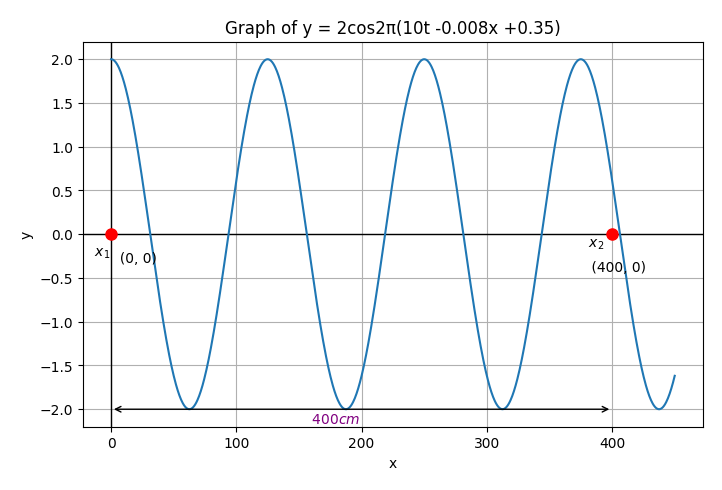
\includegraphics[width=\columnwidth]{ncert-physics/11/15/10/figs/graph1.png}
\captionsetup{justification=centering}
\caption{}
\label{fig:Graph1}
\end{figure}

\begin{figure}[!h] 
\centering
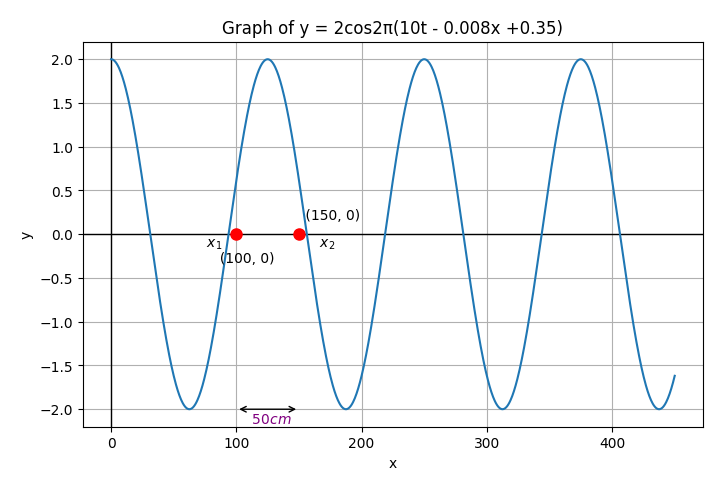
\includegraphics[width=\columnwidth]{ncert-physics/11/15/10/figs/graph2.png}
\captionsetup{justification=centering}
\caption{}
\label{fig:Graph2}
\end{figure}

\begin{figure}[!h] 
\centering
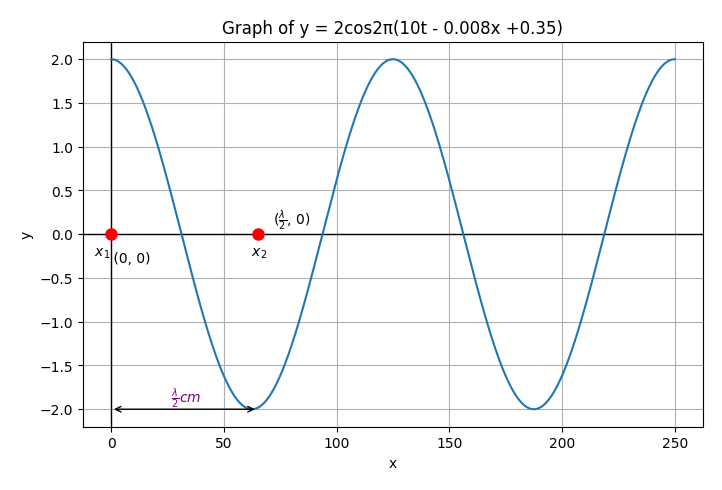
\includegraphics[width=\columnwidth]{ncert-physics/11/15/10/figs/graph3.png}
\captionsetup{justification=centering}
\caption{}
\label{fig:Graph3}
\end{figure}

\begin{figure}[!h] 
\centering
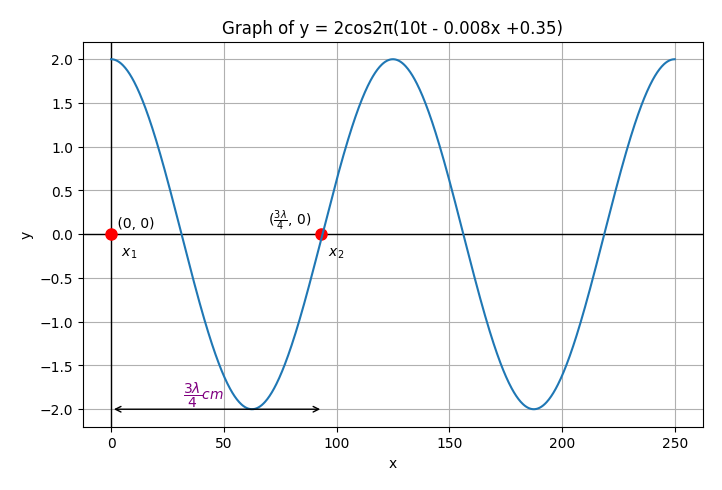
\includegraphics[width=\columnwidth]{ncert-physics/11/15/10/figs/graph4.png}
\captionsetup{justification=centering}
\caption{}
\label{fig:Graph4}
\end{figure}

